\section{插入图片和表格}
\subsection{插入图片}
利用graphicx宏包提供的$\backslash$ includegraphics命令。比如在 TeX 源文件同目录下,
有名为 a.jpg 的图片,可以用这样的方式将它插入到输出文档中:
当然也可以在导言部分使用$\backslash$graphicspath\{路径\}来制定图片的搜索路径.
图片可能很大,超过了输出文件的纸张大小,或者干脆就是你自己觉得输出的效果不爽。
这时候可以用 $\backslash$includegraphics 控制序列的可选参数来控制。
比如$\backslash$includegraphics [ width = .8$\backslash$ textwidth ] \{a.jpg\}。
这样图片的宽度会被缩放至页面宽度的百分之八十,图片的总高度会按比例缩放。
其他的功能可以查看该包的文档。

\subsection{插入表格}
tabular环境提供了最简单的表格功能,用 $\backslash$hline 命令表示横线,
在列格式中用 | 表示竖线;用 \& 来分列,
用 $\backslash$$\backslash$ 来换行;
每列可以采用居左、居中、居右等横向对齐方式,分别用 l、c、r 来表示。

\begin{equation*}
    \begin{tabular}{|l|c|r|}
        \hline
       操作系统& 发行版& 编辑器\\
        \hline
       Windows & MikTeX & TexMakerX \\
        \hline
       Unix/Linux & teTeX & Kile \\
        \hline
       Mac OS & MacTeX & TeXShop \\
        \hline
       通用& TeX Live & TeXworks \\
        \hline
       \end{tabular}
\end{equation*}
有时候我们需要列出一些总结,可以使用itemize环境与$\backslash$item。而item后面可以跟一个方括号,
中括号内的东西就替换掉默认的黑点,根据需求添加序号,比如下面这个例子
\begin{itemize}
  \item 第一条        
  \item[(2)] 第二条      
\end{itemize}
或者使用下面的enumerate环境紧接方括号内label=$($ $\backslash$arabic*$)$配上自动标号
\begin{enumerate}[label=(\arabic*)]
  \item 自动标号       
\end{enumerate}
除此之外,可以使用 booktabs 宏包中的
$\backslash$toprule、$\backslash$midrule和$\backslash$bottomrule命令。
这些命令提供了更好的表格线样式,并且专门用于创建三横线表格。
\begin{equation*}
    \begin{tabular}{ccccc}
        \toprule
        姓名 & 数学 & 语文 & 英语 & 总分 \\
        \midrule
        张三 & 85 & 90 & 75 & 250 \\
        李四 & 95 & 85 & 80 & 260 \\
        王五 & 80 & 85 & 85 & 250 \\
        \bottomrule
    \end{tabular}
\end{equation*}
当然我们还可以使用插入图片的方式来进行表格的进一步控制,比如在下方添加表的名字,
可以使$\backslash$caption*\{\}的方式从而取消图片的标序,
两个表之间可以手动使用$\backslash$vspace\{2cm\}指定间隔,具体可以查看源代码
\vspace{2cm}
\begin{table}[htbp]
    \centering
    \begin{tabular}{ccccc}
        \toprule
        姓名 & 数学 & 语文 & 英语 & 总分 \\
        \midrule
        张三 & 85 & 90 & 75 & 250 \\
        李四 & 95 & 85 & 80 & 260 \\
        王五 & 80 & 85 & 85 & 250 \\
        \bottomrule
    \end{tabular}
    % 使用*从而取消图片的标序
    \caption*{成绩表}
    \label{tab:grade}
\end{table}

% 或者使用下面的enumerate环境的方法自动标号
% \begin{enumerate}[label=(\arabic*)]
%   \item         
% \end{enumerate}
\subsection{浮动体}
插图和表格通常需要占据大块空间,所以在文字处理软件中我们经常需要调整他们的位置。
figure 和 table 环境可以自动完成这样的任务;
这种自动调整位置的环境称作浮动体(float) 。我们以 figure 为例。
\begin{figure}[htbp]
    \centering
    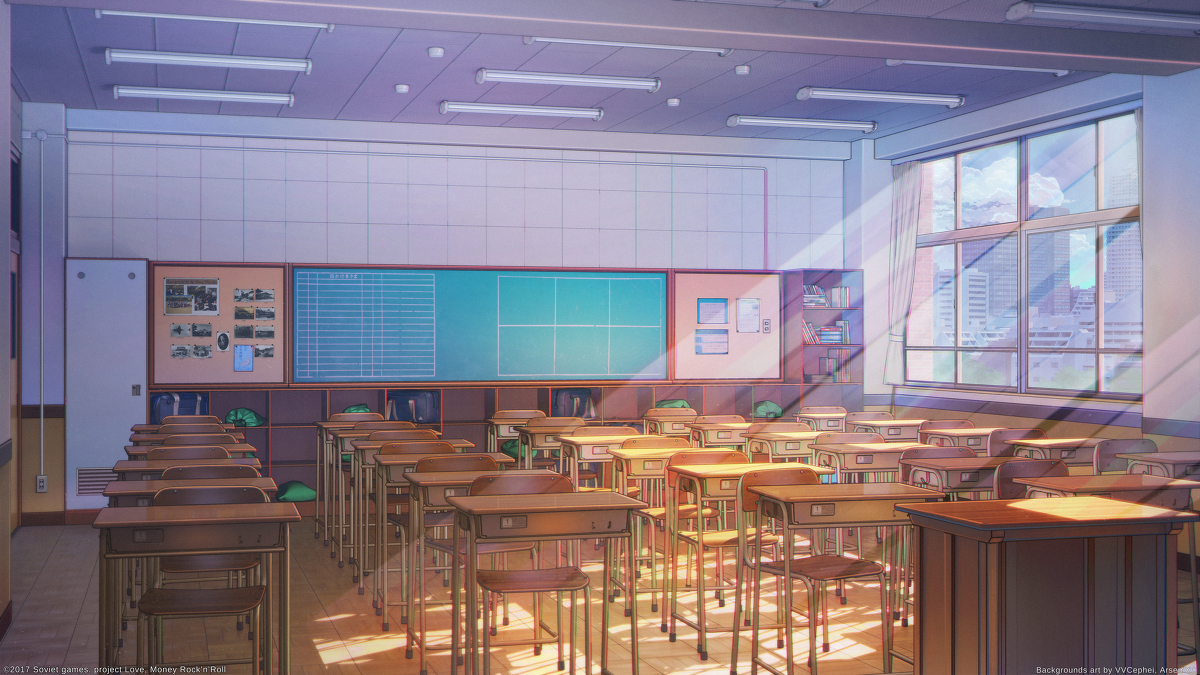
\includegraphics[width = .8\textwidth]{classroom.png}
    \caption{有图有真相}
    \label{fig:myphoto}
\end{figure}
htbp 选项用来指定插图的理想位置,
这几个字母分别代表 here, top, bottom, float page,
也就是就这里、页顶、页尾、浮动页(专门放浮动体的单独页面或分栏)。
$\backslash$centering 用来使插图居中;
$\backslash$caption 命令设置插图标题,
LaTeX 会自动给浮动体的标题加上编号。注意$\backslash$label 应该放在标题命令之后。
但是实际上浮动图片的问题并非想象中的简单,这里碍于时间限制暂时写到这里。
补充一点,如果想让两个图片同行显示可以使用$\backslash$subfigure,效果如下
\begin{figure}[htbp]
    \centering
    \begin{subfigure}[b]{0.45\textwidth}
        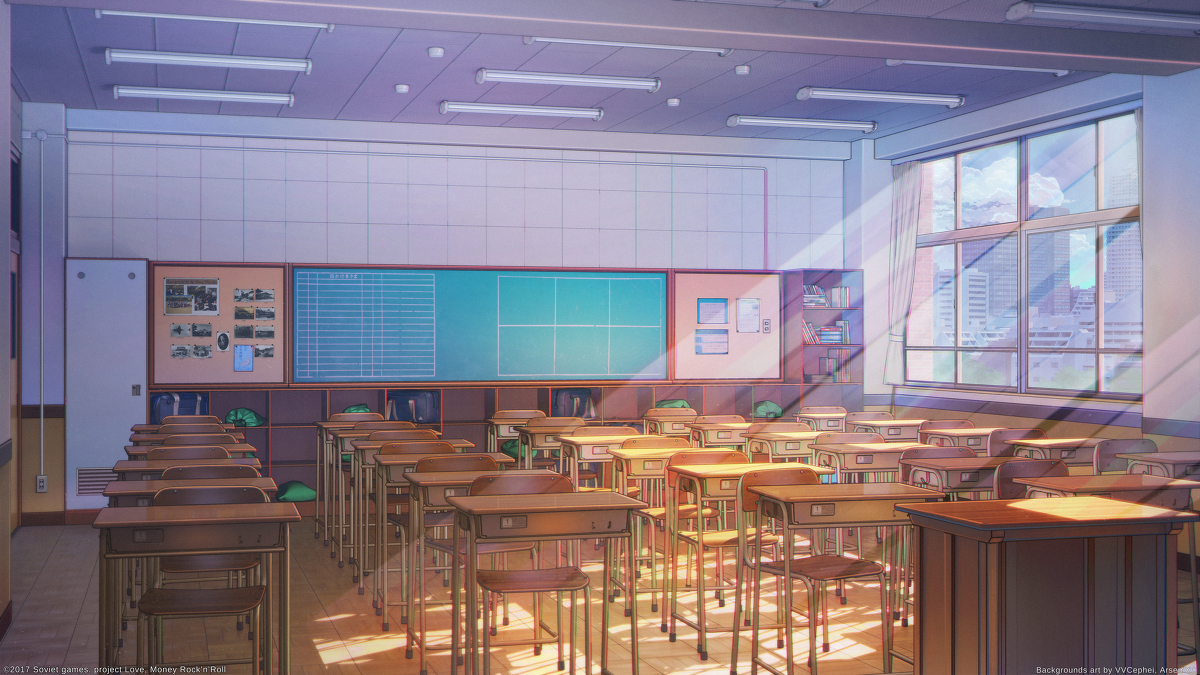
\includegraphics[width=\textwidth]{classroom.png}
        % \caption{}
        \label{fig:image1}
    \end{subfigure}
    \hfill
    \begin{subfigure}[b]{0.45\textwidth}
        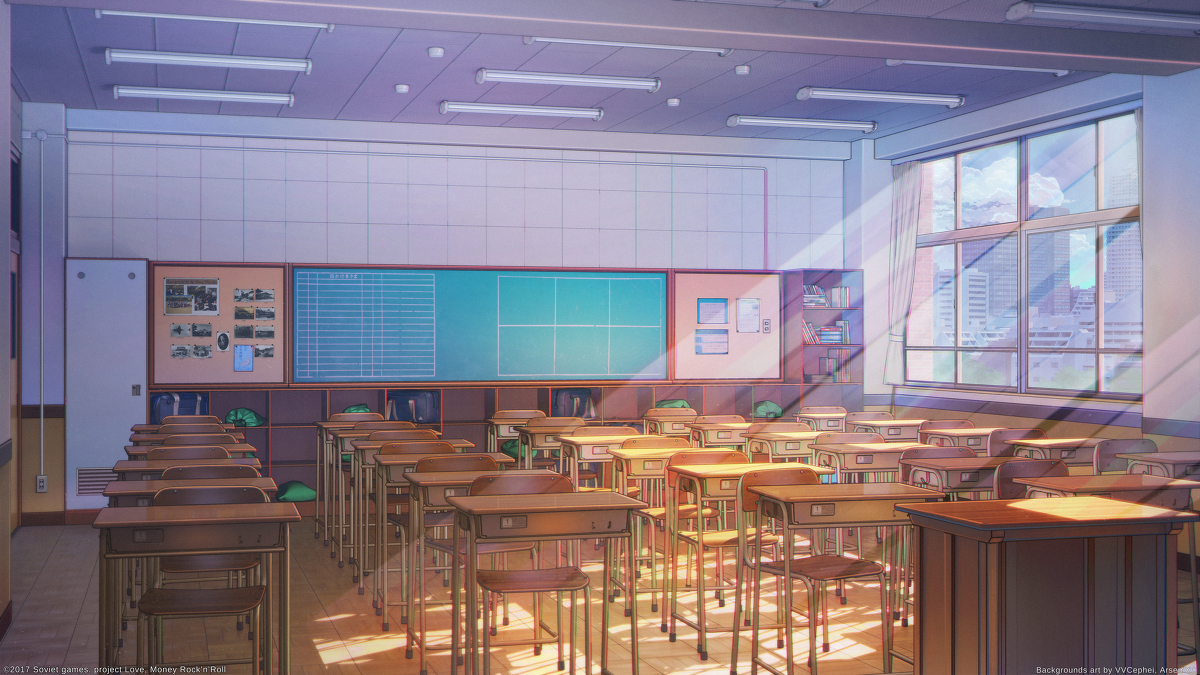
\includegraphics[width=\textwidth]{classroom.png}
        % \caption{}
        \label{fig:image2}
    \end{subfigure}
    \caption{有图有真相2}
    \label{fig:twosubfigs004}
\end{figure}